In this section we will look at several well documented marine heat waves and analyse both our sea surface and chlorophyll concentration data in a local spatial grid.

\subsection{Northwest Atlantic Ocean (2012)}

During 2012 the Northwest Atlantic Ocean saw it's largest event on record, being $2.5-0.3^\circ$C warmer than average for 226 days in the most affected region.

\begin{figure}[H]
\centering
    \textbf{37$^{\circ}$N 287$^{\circ}$E}\par
    \makebox[\textwidth][c]{
        \includegraphics[width=0.75\textwidth, angle =0]{Chapter3/NorthWestAtlantic2012/NwAtlantic.png}
        }
            \caption{A figure of SST at 37$^{\circ}$N 287$^{\circ}$E where recorded temperatures are indicated by the black line, expected temperatures (climatology) is indicated by the blue dashed line and 90th percentile temperatures are indicated by the red dotted line. Hence, the filled colour area indicates MHW days, where the darker the shade, the higher the intensity of the MHW. \cite{MHWtracker}}
            \label{fig:NwAtlantic}
\end{figure}

\noindent Looking at \autoref{fig:NwAtlantic}, we can the MHW started just after April, 2012 and continued onto August 2012 lasting around 200 days in the region we are investigating, just east of Virginia, USA.
\\\\
To begin investigating the impacts this MHW had on the health of phytoplankton we can use our Chlorophyll concentration data for the same location and build a ARIMA model, we can then compare the raw data to our model to see if the MHW causes any anomalies.
\\\\
Looking at \autoref{fig:NwAtlanticTS}, we can see the recorded chlorophyll concentration is lower than the ARIMA model from the second month in. This could be due to the MHW period showed at the start of 2012 in \autoref{fig:NwAtlantic} where SST where as high as 20 Celsius. The raw data than continues to be below the model till around late September when there is a very sharp increase in chlorophyll concentration which goes considerable higher than what the model predicted and at a much faster rate. This sharp increase in chlorophyll concentration hints at a chlorophyll bloom. If we again refer to \autoref{fig:NwAtlantic}, we can see a the SST begins to fall around September which could be responsible for the chlorophyll bloom. To investigate further we will analyse the annual climatology of chlorophyll concentration.

\begin{figure}[H]
\centering
    \makebox[\textwidth][c]{
        \includegraphics[width=0.5\textwidth, angle =-90]{Chapter3/NorthWestAtlantic2012/Data_37N287E_Chl_TS.eps}
        }
            \caption{A figure of our ARIMA model calculated using our chlorophyll data set and our raw data for 37$^{\circ}$N 287$^{\circ}$E}
            \label{fig:NwAtlanticTS}
\end{figure}

Looking at \autoref{fig:NwAtlanticCl} we can see how the maximum chlorophyll concentration is often seen in the first six months, but during the year of our heatwave the peak came much later in the year. Despite the recorded SST following roughly the same shape as SST climatology plot indicted by the blue dashed line in \autoref{fig:NwAtlantic}. This further shows the anomalous behaviour. 

\begin{figure}[H]
\centering
    \makebox[\textwidth][c]{
        \includegraphics[width=0.5\textwidth, angle =-90]{Chapter3/NorthWestAtlantic2012/Data_37N287E_Chl_Climatology.eps}
        }
            \caption{Annual climatology for chlorophyll concentration at 37$^{\circ}$N 287$^{\circ}$E}
            \label{fig:NwAtlanticCl}
\end{figure}